
\documentclass[twoside]{article}

% Set the document margins
\usepackage[top=1.00in, bottom=1.00in, left=1.00in, right=1.00in, columnsep=20pt]{geometry}
\usepackage{graphicx}

\title{Moller Scattering in 2015 Engineerin Run @ 1.056 GeV}
\date{November 1, 2015}
\author{Omar Moreno \\
        Santa Cruz Institute for Particle Physics \\
        University of California, Santa Cruz
}

\begin{document}

    \maketitle

    \begin{abstract}
        Short abstract goes here ...
    \end{abstract}

    \section*{Introduction}

    \section*{Theory}

    \section*{Datasets}

    \section*{Event Selection}

        The following criteria were used to select Moller candidates: 
            \begin{itemize}
                \item Select two Ecal clusters within a 1.6 ns window, in opposite detector volumes.
            \end{itemize}
        
            \begin{figure}
                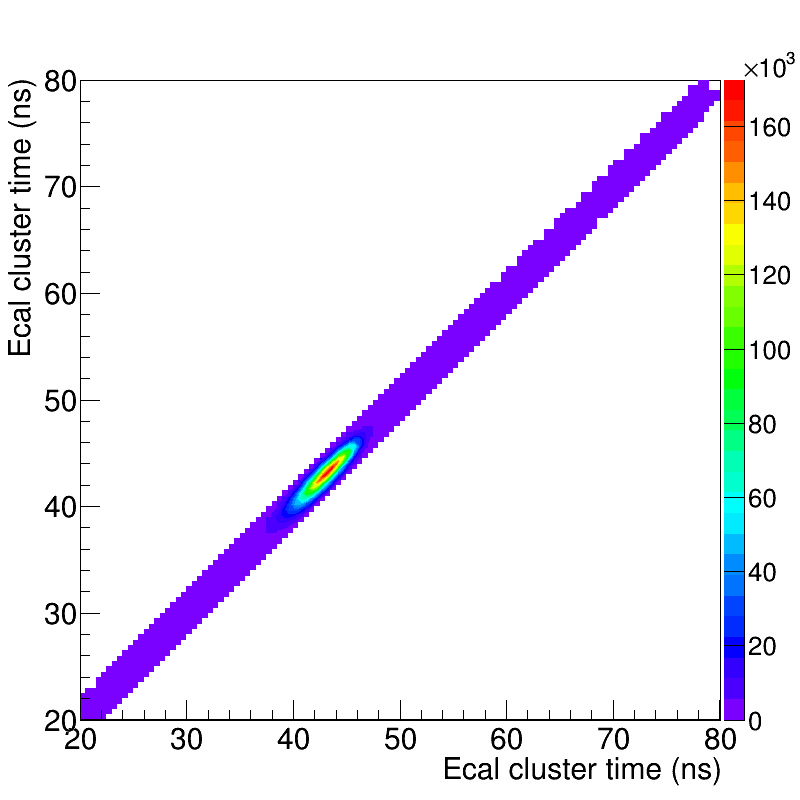
\includegraphics[width=.5\textwidth]{figures/20151102_cluster_pair_time.png}
            \end{figure}

    \section*{Conclusion}

\end{document}
